\documentclass{article}
\usepackage[utf8]{inputenc}

\usepackage[paperwidth=8.5in, paperheight=11in, top=1in, bottom=.5in, left=.5in, right=.5in]{geometry}
\usepackage{fancyhdr, graphicx,tikz,amsmath,multicol,paracol,pgfplots}
\usepackage[inline]{enumitem}
\pgfplotsset{compat=1.18}


\pagestyle{fancy}
\lhead{\large{\textbf{Module 1: Equations, Inequalities, and Applications - Readiness Assurance Test}}}
\chead{}
\rhead{}
\lfoot{}
\cfoot{}
%\rfoot{\thepage/\pageref{LastPage} }
\setlength{\headheight}{14pt} %added in bc warning

%%% LIST ANSWER KEY HERE

% 1 B
% 2 C
% 3 B
% 4 D
% 5 C
% 6 C
% 7 B
% 8 D
% 9 B
% 10 C


\begin{document}


\begin{enumerate}


% WRITE WHICH READINESS OBJECTIVE THE PROBLEM GOES WITH AS COMMENT

% \item Sample question with 4 answers in one column. (Tag correct answer with comment.)

%   \begin{enumerate}
  
%   \item first answer choice  %correct 
%   \item second answer choice
%   \item third answer choice
%   \item fourth answer choice
  
%   \end{enumerate}

% % objective description

% \item Sample question with four answers on one row. 

%   \begin{enumerate}
%   \begin{multicols}{4}
%   \item first answer choice  %correct 
%   \item second answer choice
%   \item third answer choice
%   \item fourth answer choice
%   \end{multicols}
%   \end{enumerate}


%Plot points on the coordinate plane.

\item A point is graphed on the coordinate plane. Which ordered pair represents this point?

        \begin{center}
        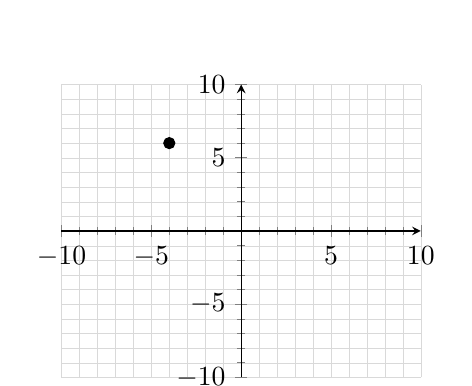
\begin{tikzpicture}
        \begin{axis}[
                height=5.3cm,
                axis lines=center,
                grid=both,
                grid style={line width=.05pt, draw=gray!30},
                minor tick num=4,
                xtick={-10,-5,...,10},
                ytick={-10,-5,...,10},
                xmin=-10, xmax=10,
                ymin=-10, ymax=10,
                ]
                \addplot[mark=*] coordinates {(-4,6)};
        \end{axis}
        \end{tikzpicture}
        \end{center}

        \begin{enumerate}
        \begin{multicols}{4}
          \item $(6,-4)$  %reversed order
          \item $(-4,6)$  %correct 
          \item $(4,-6)$  %reversed signs
          \item $(-6,-4)$ %reversed order and signs
        \end{multicols}
        \end{enumerate}


% Determine whether a given value is a solution to an equation.

\item For which equation below is $x=-2$ a solution?

        \begin{enumerate}
        \begin{multicols}{4}
          
          \item $-3x+14=4x$
          \item $5x-4=3x-3$
          \item $2+6x=2x-6$  %correct 
          \item $4-3x=3-5x$
          
        \end{multicols}
        \end{enumerate}

% Solve two step linear equations.

\item Solve for $w$ in the equation  \(4-12w=-32 \).

        \begin{enumerate}
        \begin{multicols}{4}
          \item $w=2$
          \item $w=3$ %correct
          \item $w=4$
          \item $w=5$
          
        \end{multicols}
        \end{enumerate}

% Use interval notation.

\item Write the interval $x<-2$ in interval notation. 

        \begin{enumerate}
        \begin{multicols}{4}
          \item $(-2,-\infty)$
          \item $[-2,-\infty)$
          \item $(-\infty,-2]$
          \item $(-\infty,-2)$ %correct
        \end{multicols}
        \end{enumerate}

% Find the absolute value of real numbers.

\item Evaluate $|8-2(7)|$.

        \begin{enumerate}
        \begin{multicols}{4}
          \item $-22$
          \item $-6$
          \item $6$ %correct
          \item $22$
        \end{multicols}
        \end{enumerate}


% Use the Pythagorean Theorem to find side lengths of right triangles AND Simplify square roots of positive numbers.

\item A right triangle has one leg of length $7$ inches and its hypotenuse is $15$ inches. What is the length of the other leg of the triangle? Simplify your answer.

        \begin{enumerate}
        \begin{multicols}{4}
          
          \item $\sqrt{176}$ inches %not simplified
          \item $\sqrt{274}$ inches %treated 7 & 15 both as legs
          \item $4\sqrt{11}$ inches %correct
          \item $2\sqrt{44}$
        \end{multicols}
        \end{enumerate}


% Factor quadratic equations.

\item Factor $x^2-4x-12$.

        \begin{enumerate}
        \begin{multicols}{4}
          \item $(x-2)(x+6)$
          \item $(x+2)(x-6)$  %correct
          \item $(x-3)(x+4)$
          \item $(x+3)(x-4)$
        \end{multicols}
        \end{enumerate}



% Solve one-step problems involving distance, rate, and time.

\item A train travels for $6$ hours at a constant speed. If the total distance covered was $1860$ kilometers, what was the train's speed?

        \begin{enumerate}
        \begin{multicols}{4}
          \item $11{,}160$ km/h %multiplied
          \item $0.003$ km/h %divided the opposite way
          \item $1866$ km/h %added
          \item $310$ km/h  %correct
        \end{multicols}
        \end{enumerate}

% Use the percent equation.

\item A school has $875$ brownies for a bake sale, $48\%$ of which include walnuts. How many brownies have walnuts?

        \begin{enumerate}
        \begin{multicols}{4}
          \item $410$
          \item $420$  %correct
          \item $430$
          \item $440$
        \end{multicols}
        \end{enumerate}

% Simplify square roots of negative numbers using i AND Simplify square roots of positive numbers.

\item Simplify $\sqrt{-90}$, using the imaginary unit $i$ as necessary.

        \begin{enumerate}
        \begin{multicols}{4}
          \item $3\sqrt{10i}$  
          \item $-3i\sqrt{10}$ 
          \item $3i\sqrt{10}$ %correct
          \item $-3\sqrt{10i}$ 
        
        \end{multicols}
        \end{enumerate}



 
  

\end{enumerate}


\end{document}